\section{Resultados}\label{sec:resultados}

\subsection{Caudal de Ventilación}

Aplicando la Ec. (\ref{eq:caudal}) con un volumen efectivo de 320 m$^3$ y 12 renovaciones de aire por hora, se obtiene un caudal de ventilación de 64.0 m$^3$/min. La equivalencia en otras unidades se presenta en la Tabla \ref{tab:flow_results}.

\begin{table}[htbp]
	\centering
	\caption{Resultados del caudal de ventilación}
	\label{tab:flow_results}
	\setcounter{itemcount}{0}
	\begin{tabularx}{\textwidth}{@{}NXllc@{}}
		\toprule
		\multicolumn{1}{c}{\textbf{Item}} & \textbf{Magnitud} & \textbf{Valor} & \textbf{Unidad} & \textbf{Referencia} \\
		\midrule
		& Caudal volumétrico & 64.0 & m$^3$/min & Ec. (\ref{eq:caudal}) \\
		& Caudal volumétrico & 3 840 & m$^3$/h & Conversión \\
		& Caudal volumétrico & 2 260.1 & CFM & Conversión \\
		& Caudal en unidades SI & 1.0667 & m$^3$/s & Conversión \\
		\bottomrule
	\end{tabularx}
\end{table}

\subsection{Potencia del Ventilador}

La Tabla \ref{tab:fan_power} resume los resultados de potencia para diferentes escenarios de presión total a las condiciones del sitio (Cajicá, $\rho$ = 0.88 kg/m$^3$). El escenario de diseño corresponde a 165 Pa, que incluye las pérdidas por filtración MERV 13-14 cargada y la pérdida de descarga libre de las rejillas; el punto equivalente de catálogo (densidad estándar 1.2 kg/m$^3$) es 3 840 m$^3$/h a 225 Pa \cite{dml_hd_vent_001,dml_hd_filt_001}.

\begin{table}[htbp]
	\centering
	\caption{Resultados de potencia del ventilador}
	\label{tab:fan_power}
	\setcounter{itemcount}{0}
	\begin{tabularx}{\textwidth}{@{}NXllc@{}}
		\toprule
		\multicolumn{1}{c}{\textbf{Item}} & \textbf{Escenario} & \textbf{Presión Total} & \textbf{Potencia} & \textbf{Referencia} \\
		& & \textbf{(Pa)} & \textbf{(kW)} & \\
		\midrule
		& MERV limpio & 70 & 0.136 & Ec. (\ref{eq:potencia}) \\
		& Diseño (MERV cargado) & 165 & 0.320 & Ec. (\ref{eq:potencia}) \\
		& HEPA limpio (referencia histórica) & 261 & 0.506 & Ec. (\ref{eq:potencia}) \\
		& HEPA cargado (referencia histórica) & 611 & 1.185 & Ec. (\ref{eq:potencia}) \\
		& Motor provisional & -- & 0.75 HP & Criterio de diseño \\
		\bottomrule
	\end{tabularx}
\end{table}

\subsection{Área de Impulsión del Ventilador}

Con una velocidad de impulsión de 8 m/s, el área de boca del ventilador es 0.1333 m$^2$, lo cual corresponde a un diámetro equivalente de 412 mm y un radio de 206.0 mm. Los resultados se presentan en la Tabla \ref{tab:inlet_results}.

\begin{table}[htbp]
	\centering
	\caption{Resultados del área de impulsión del ventilador}
	\label{tab:inlet_results}
	\setcounter{itemcount}{0}
	\begin{tabularx}{\textwidth}{@{}NXllc@{}}
		\toprule
		\multicolumn{1}{c}{\textbf{Item}} & \textbf{Parámetro} & \textbf{Valor} & \textbf{Unidad} & \textbf{Referencia} \\
		\midrule
		& Área de impulsión & 0.1333 & m$^2$ & Ec. (\ref{eq:area_vent}) \\
		& Diámetro equivalente & 412 & mm & Ec. (\ref{eq:diametro}) \\
		& Radio equivalente & 206.0 & mm & Ec. (\ref{eq:diametro}) \\
		& Velocidad de impulsión & 8.0 & m/s & Criterio de diseño \\
		\bottomrule
	\end{tabularx}
\end{table}

\subsection{Rejillas de Exfiltración}

Para una velocidad de exfiltración de 3.0 m/s, el área neta total requerida es 0.3556 m$^2$. Distribuida en tres rejillas, cada una debe tener un área neta de 0.1185 m$^2$. Las dimensiones calculadas son 353.2 mm de alto por 335.5 mm de ancho. La Tabla \ref{tab:outlet_results} resume estos resultados.

\begin{table}[htbp]
	\centering
	\caption{Resultados de las rejillas de exfiltración}
	\label{tab:outlet_results}
	\setcounter{itemcount}{0}
	\begin{tabularx}{\textwidth}{@{}NXllc@{}}
		\toprule
		\multicolumn{1}{c}{\textbf{Item}} & \textbf{Parámetro} & \textbf{Valor} & \textbf{Unidad} & \textbf{Referencia} \\
		\midrule
		& Número de rejillas & 3 & unidades & Criterio de diseño \\
		& Velocidad de exfiltración & 3.0 & m/s & Criterio de diseño \\
		& Área neta total & 0.3556 & m$^2$ & Ec. (\ref{eq:area_exfil}) \\
		& Área neta por rejilla & 0.1185 & m$^2$ & División equitativa \\
		& Altura de rejilla & 353.2 & mm & Criterio de diseño \\
		& Ancho de rejilla & 335.5 & mm & Criterio de diseño \\
		\bottomrule
	\end{tabularx}
\end{table}

\subsection{Datos para Modelado CFD}

La Tabla \ref{tab:cfd_boundaries} presenta las condiciones de contorno recomendadas para el modelo CFD.

\begin{table}[htbp]
	\centering
	\caption{Condiciones de contorno para el modelo CFD}
	\label{tab:cfd_boundaries}
	\setcounter{itemcount}{0}
	\begin{tabularx}{\textwidth}{@{}Nlllc@{}}
		\toprule
		\multicolumn{1}{c}{\textbf{Item}} & \textbf{Elemento} & \textbf{Geometría} & \textbf{Dimensiones} & \textbf{Condición de Contorno} \\
		\midrule
		& Impulsión del ventilador & Círculo & $r$ = 206.0 mm & Velocity inlet, \SI{8}{m/s} \\
		& Rejilla de salida 1 & Rectángulo & 353 mm $\times$ 336 mm & Pressure outlet, \SI{0}{Pa} gauge \\
		& Rejilla de salida 2 & Rectángulo & 353 mm $\times$ 336 mm & Pressure outlet, \SI{0}{Pa} gauge \\
		& Rejilla de salida 3 & Rectángulo & 353 mm $\times$ 336 mm & Pressure outlet, \SI{0}{Pa} gauge \\
		& Paredes del laboratorio & Sólidas & Según geometría 3D & Wall, no slip \\
		\bottomrule
	\end{tabularx}
\end{table}

El balance de masas de diseño presenta una discrepancia inferior al 0.1 \%. El caudal de entrada es 1.0667 m$^3$/s, mientras que el caudal teórico de salida distribuido en tres rejillas a \SI{3}{m/s} es 3 $\times$ (0.3532 m $\times$ 0.3355 m) $\times$ \SI{3}{m/s} = 1.0665 m$^3$/s. La diferencia (0.02 \%) se debe al redondeo de dimensiones. Al imponer \texttt{pressure outlet} en las rejillas, el solver determina el caudal de exfiltración a partir del campo de presión; los resultados visuales confirman velocidades faciales del orden de \SI{3}{m/s} en las salidas.

\subsection{Resultados de la simulación CFD}

El modelo de dinámica de fluidos computacional se resolvió en Autodesk CFD con las condiciones de contorno de la Tabla \ref{tab:cfd_boundaries}: inyección como \texttt{velocity inlet} de \SI{8}{m/s} y las tres rejillas como \texttt{pressure outlet} a \SI{0}{Pa} gauge, condición que representa la descarga libre real a la atmósfera. Esta condición de salida evita la sobreespecificación del problema y permite que el caudal de descarga se determine a partir del campo de presión interior. En el régimen incompresible del modelo, los resultados se interpretan como la distribución de flujo y la ventilación del recinto. Las Figuras \ref{fig:cfd_streamlines} a \ref{fig:cfd_vectores_corte} presentan los campos de velocidad resultantes. La velocidad máxima se sitúa en torno a \SI{8}{m/s}, coherente con la inyección de diseño, mientras que las salidas presentan velocidades del orden de \SI{3}{m/s}, compatibles con el dimensionamiento de las rejillas.

\begin{figure}[htbp]
	\centering
	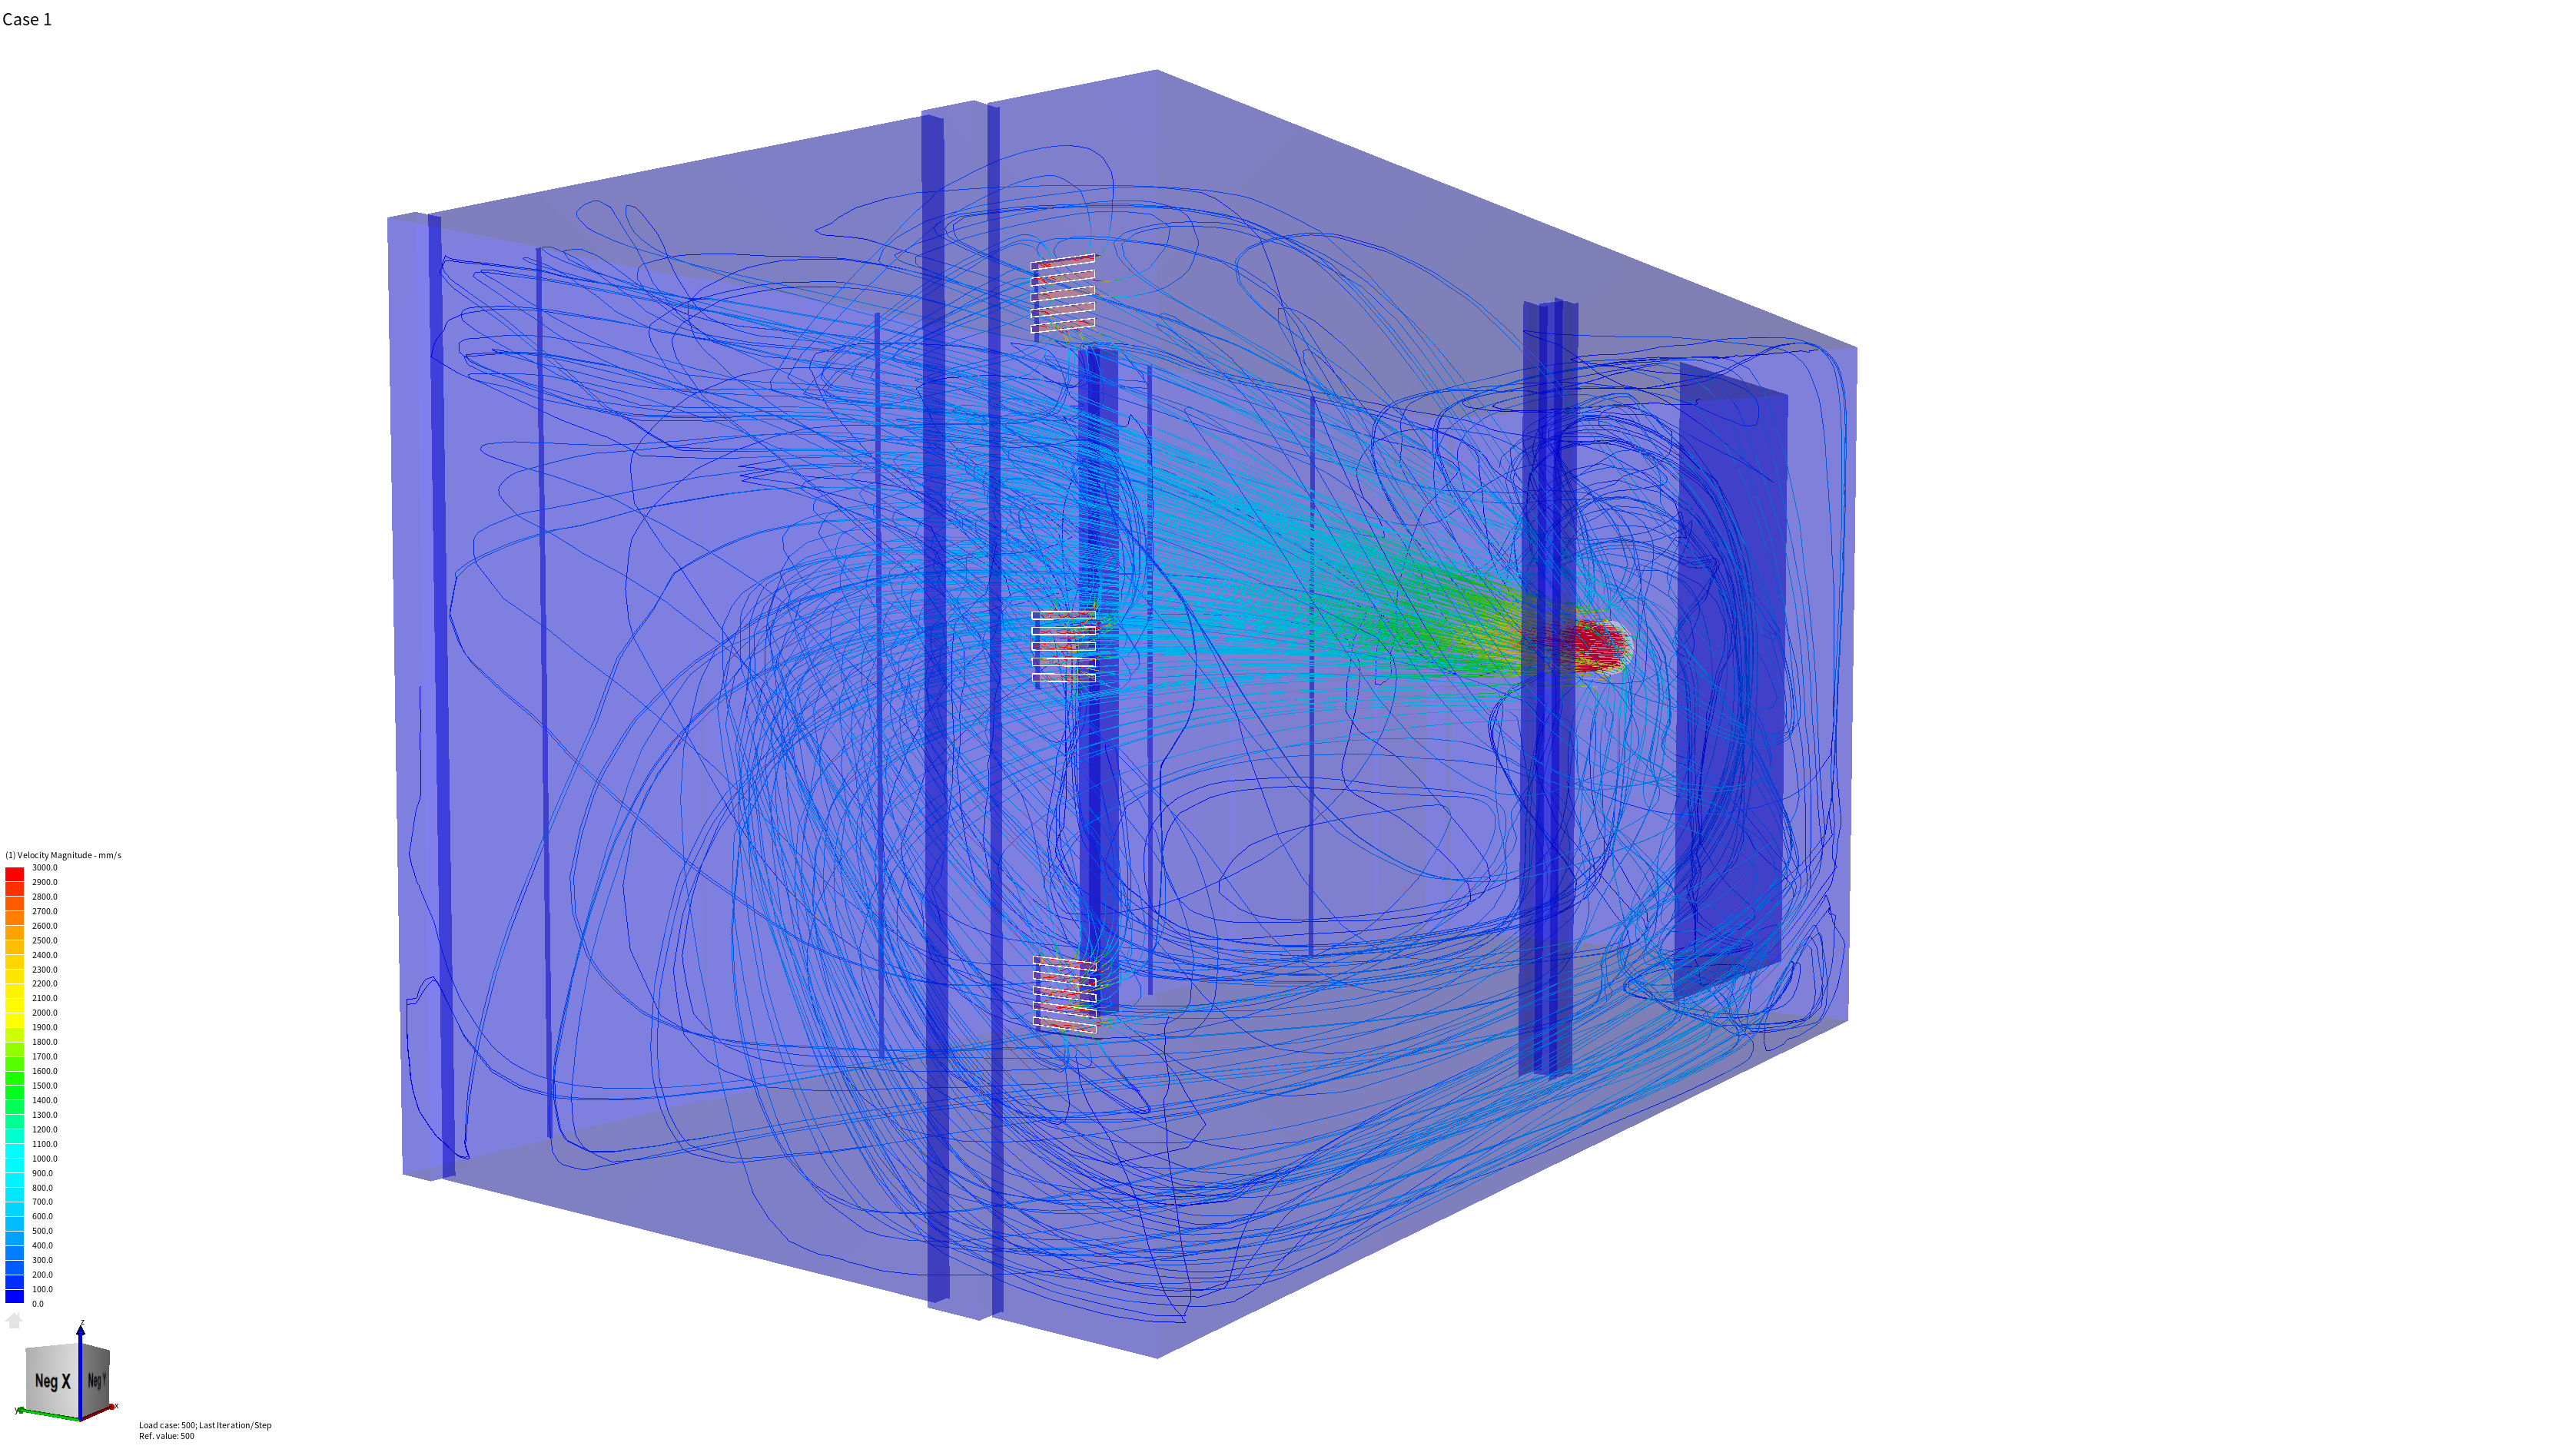
\includegraphics[width=0.92\textwidth]{figures/cfd_streamlines_3d.png}
	\caption{Líneas de corriente coloreadas por magnitud de velocidad. Vista isométrica del recinto; la inyección se localiza en el extremo derecho y la exfiltración se distribuye entre las tres rejillas del lado opuesto. Escala 0--8200~mm/s.}
	\label{fig:cfd_streamlines}
\end{figure}

\begin{figure}[htbp]
	\centering
	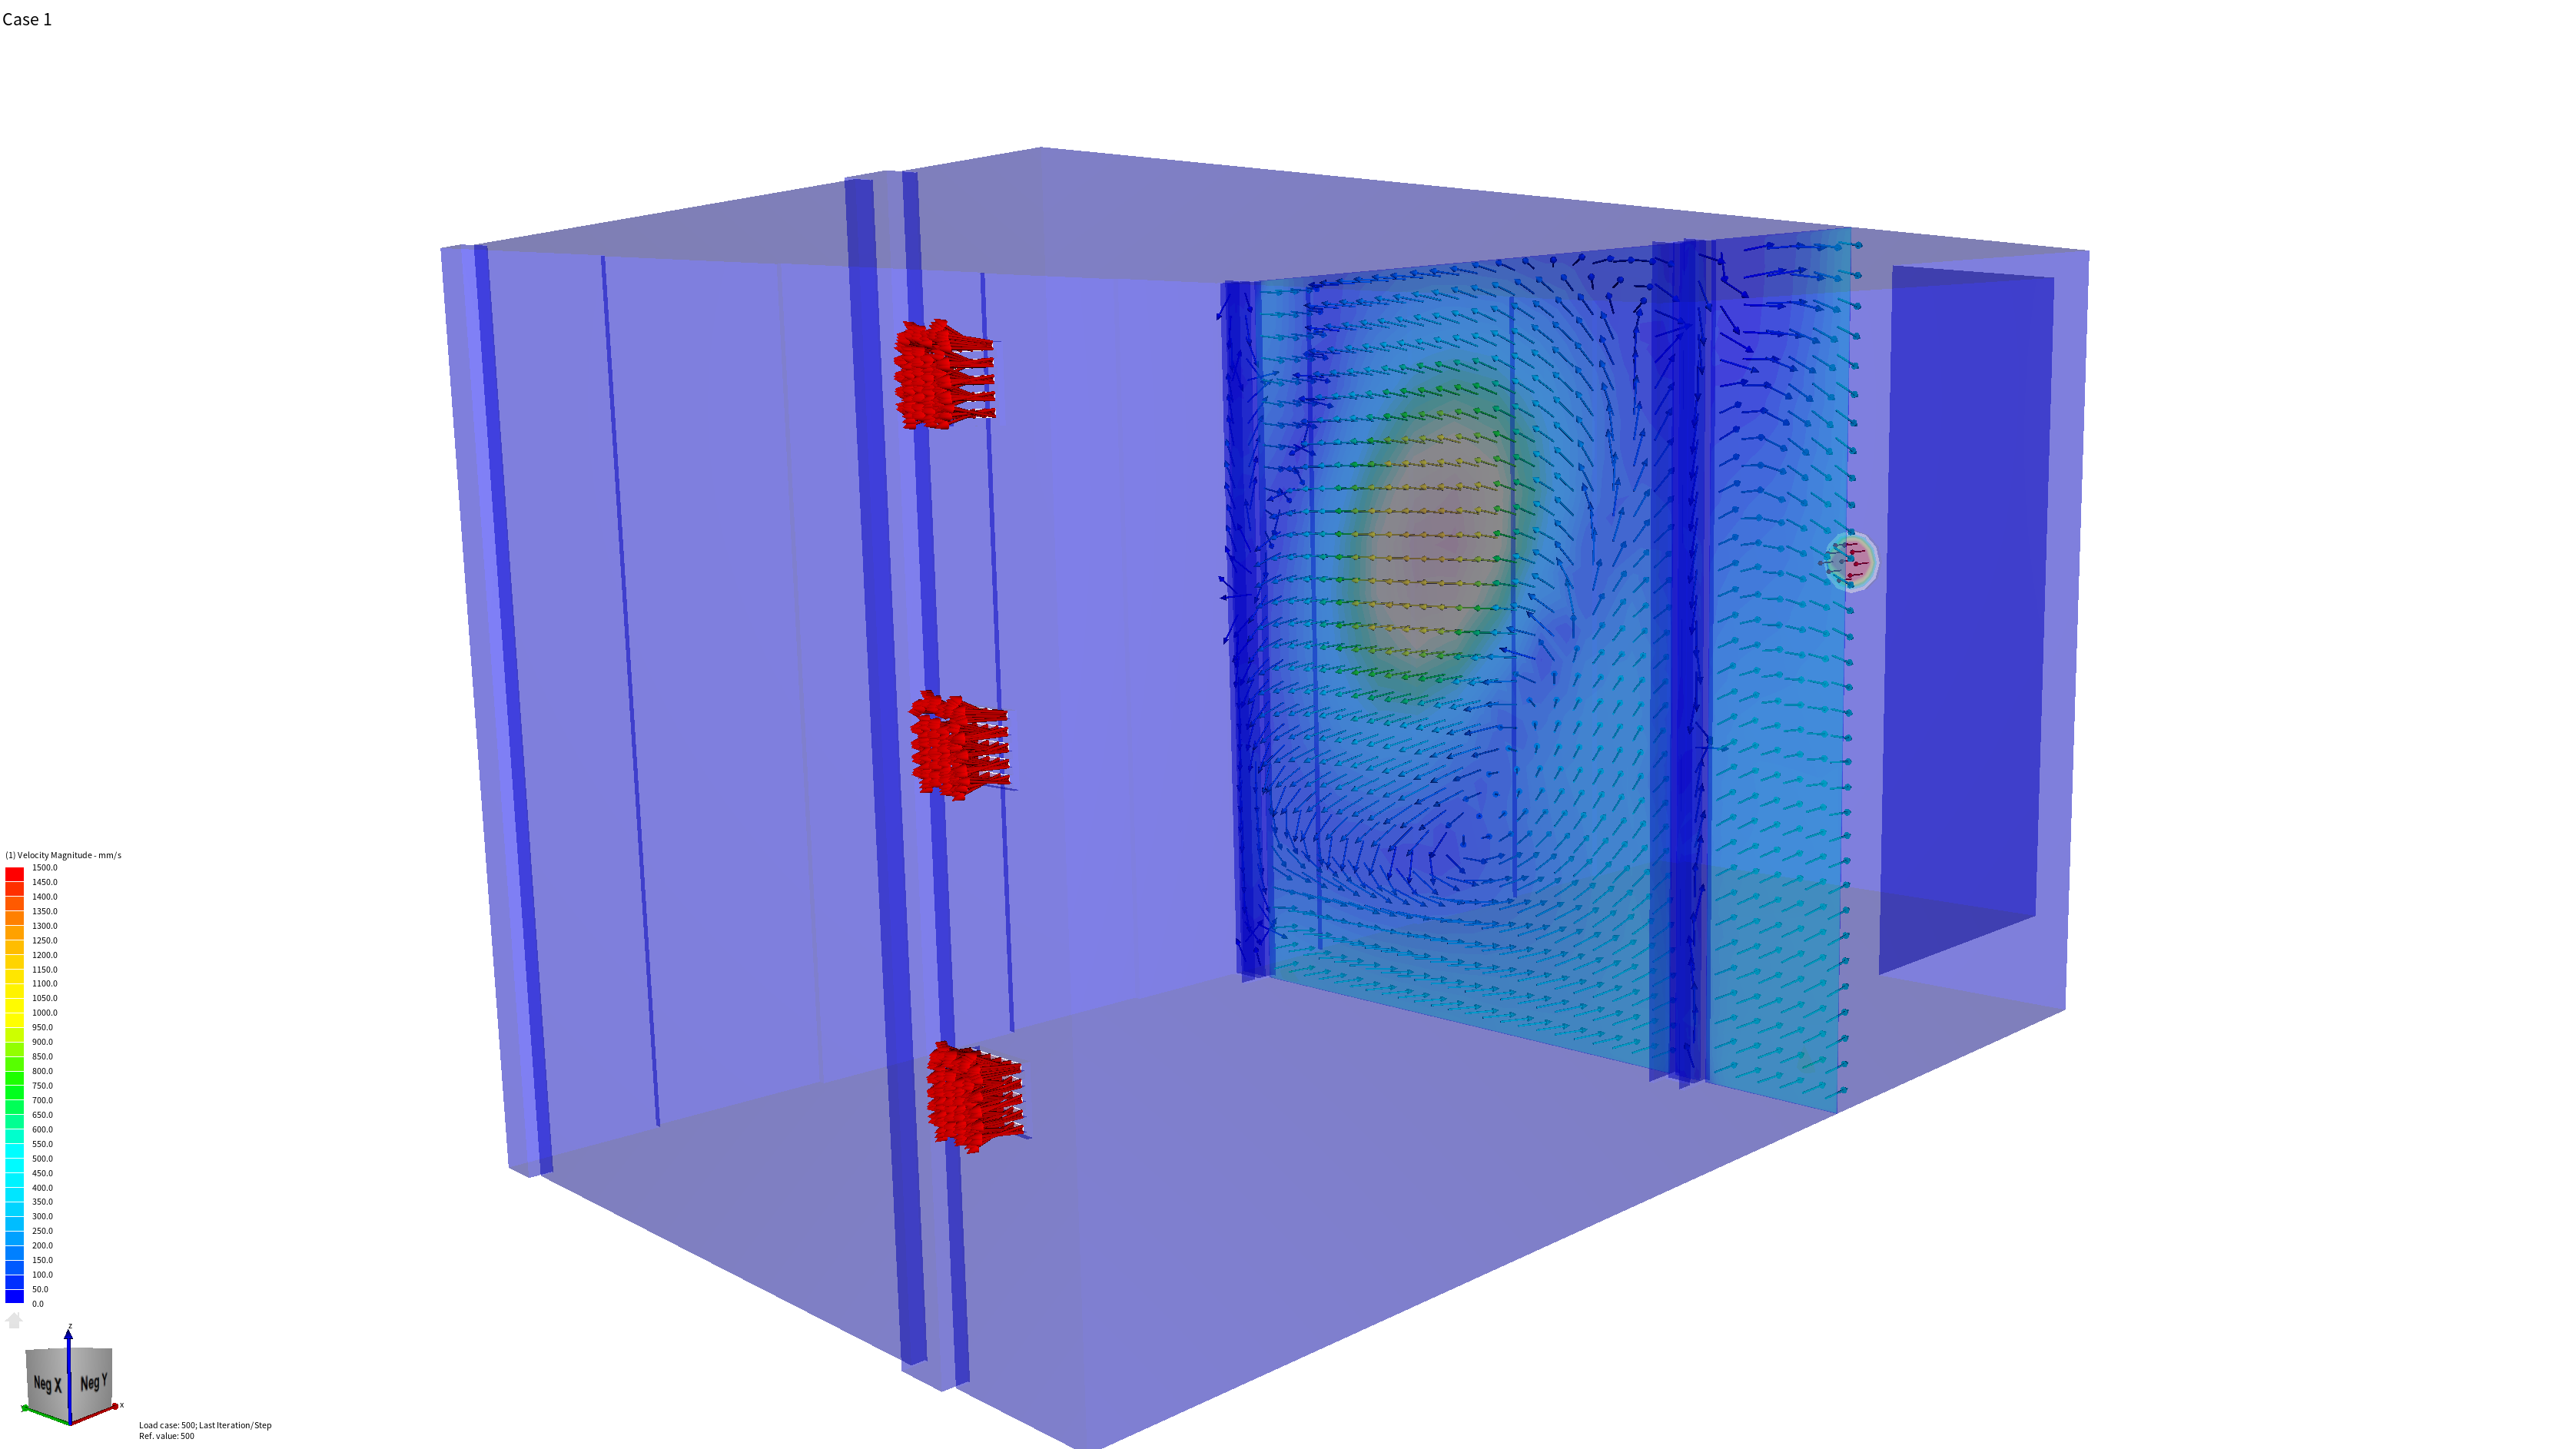
\includegraphics[width=0.92\textwidth]{figures/cfd_vectores_3d.png}
	\caption{Campo vectorial de velocidad en un corte vertical del recinto (vista isométrica). Se observa el flujo dirigido hacia las rejillas de exfiltración y la recirculación en la zona posterior.}
	\label{fig:cfd_vectores_3d}
\end{figure}

\begin{figure}[htbp]
	\centering
	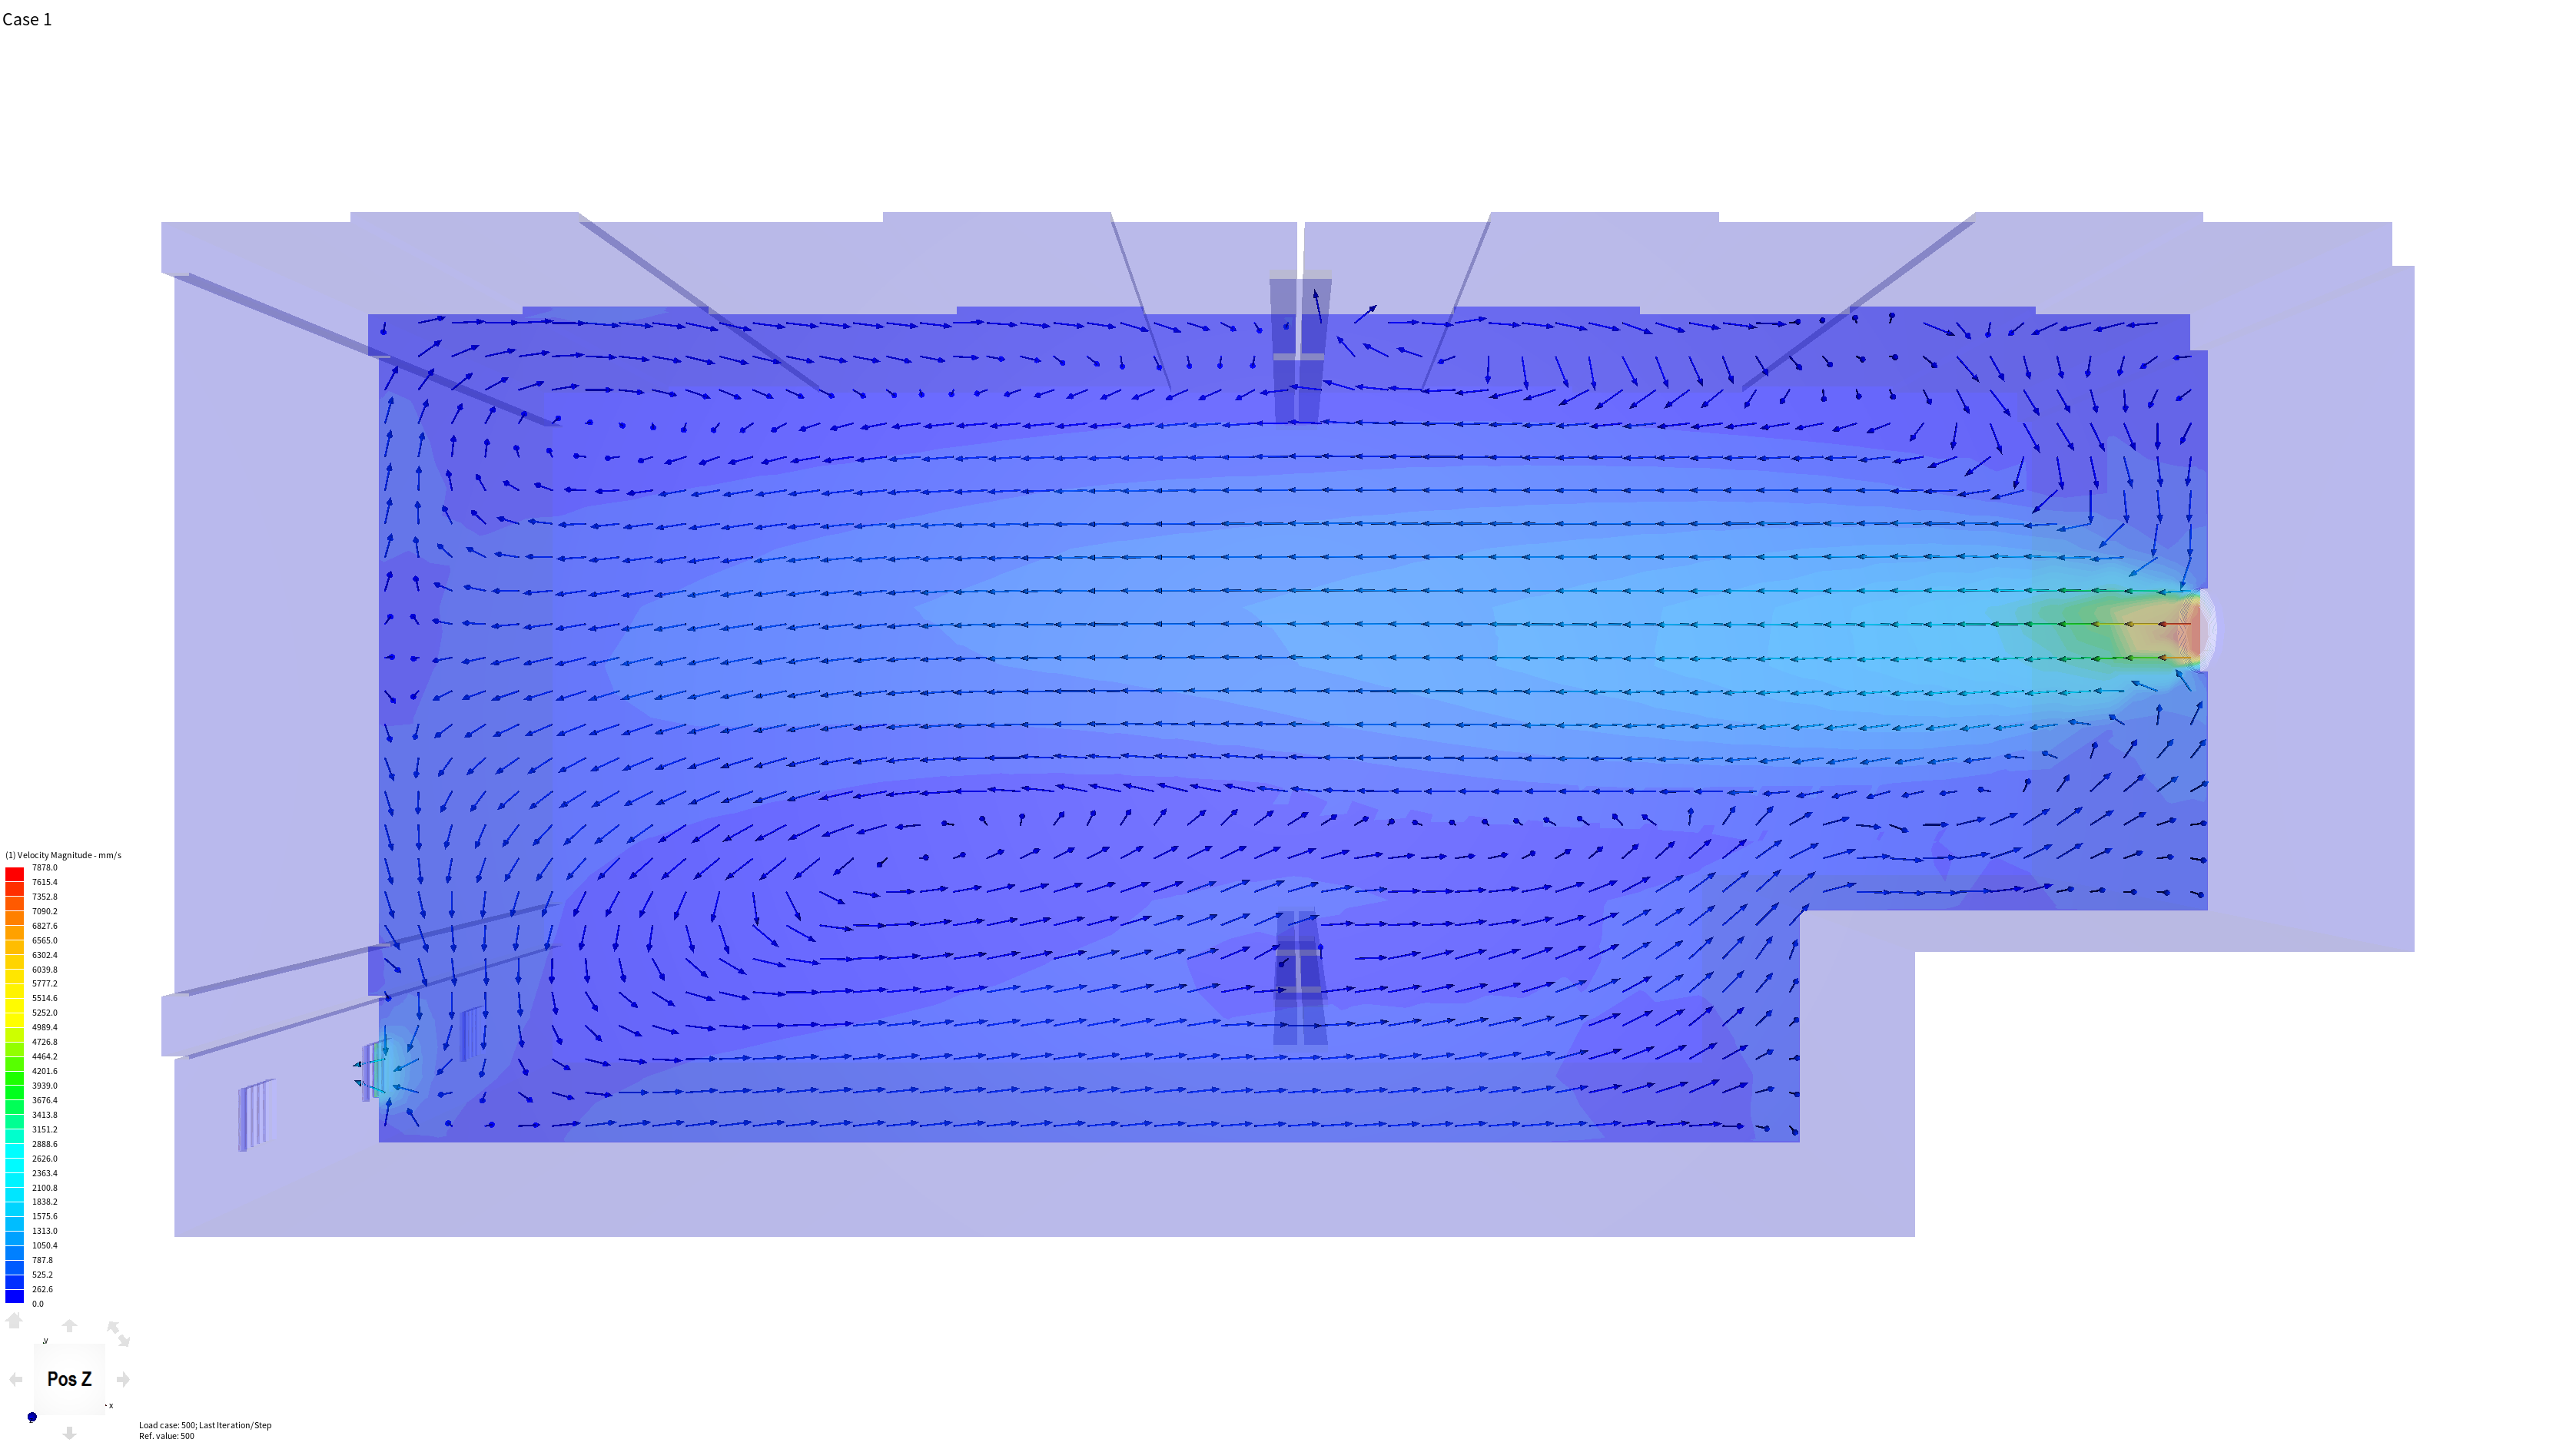
\includegraphics[width=0.92\textwidth]{figures/cfd_planta_horizontal.png}
	\caption{Campo de velocidad en plano horizontal (vista en planta). La inyección desde la derecha genera un flujo cruzado hacia las tres rejillas de la izquierda; las zonas periféricas presentan vórtices de baja velocidad.}
	\label{fig:cfd_planta_horizontal}
\end{figure}

\begin{figure}[htbp]
	\centering
	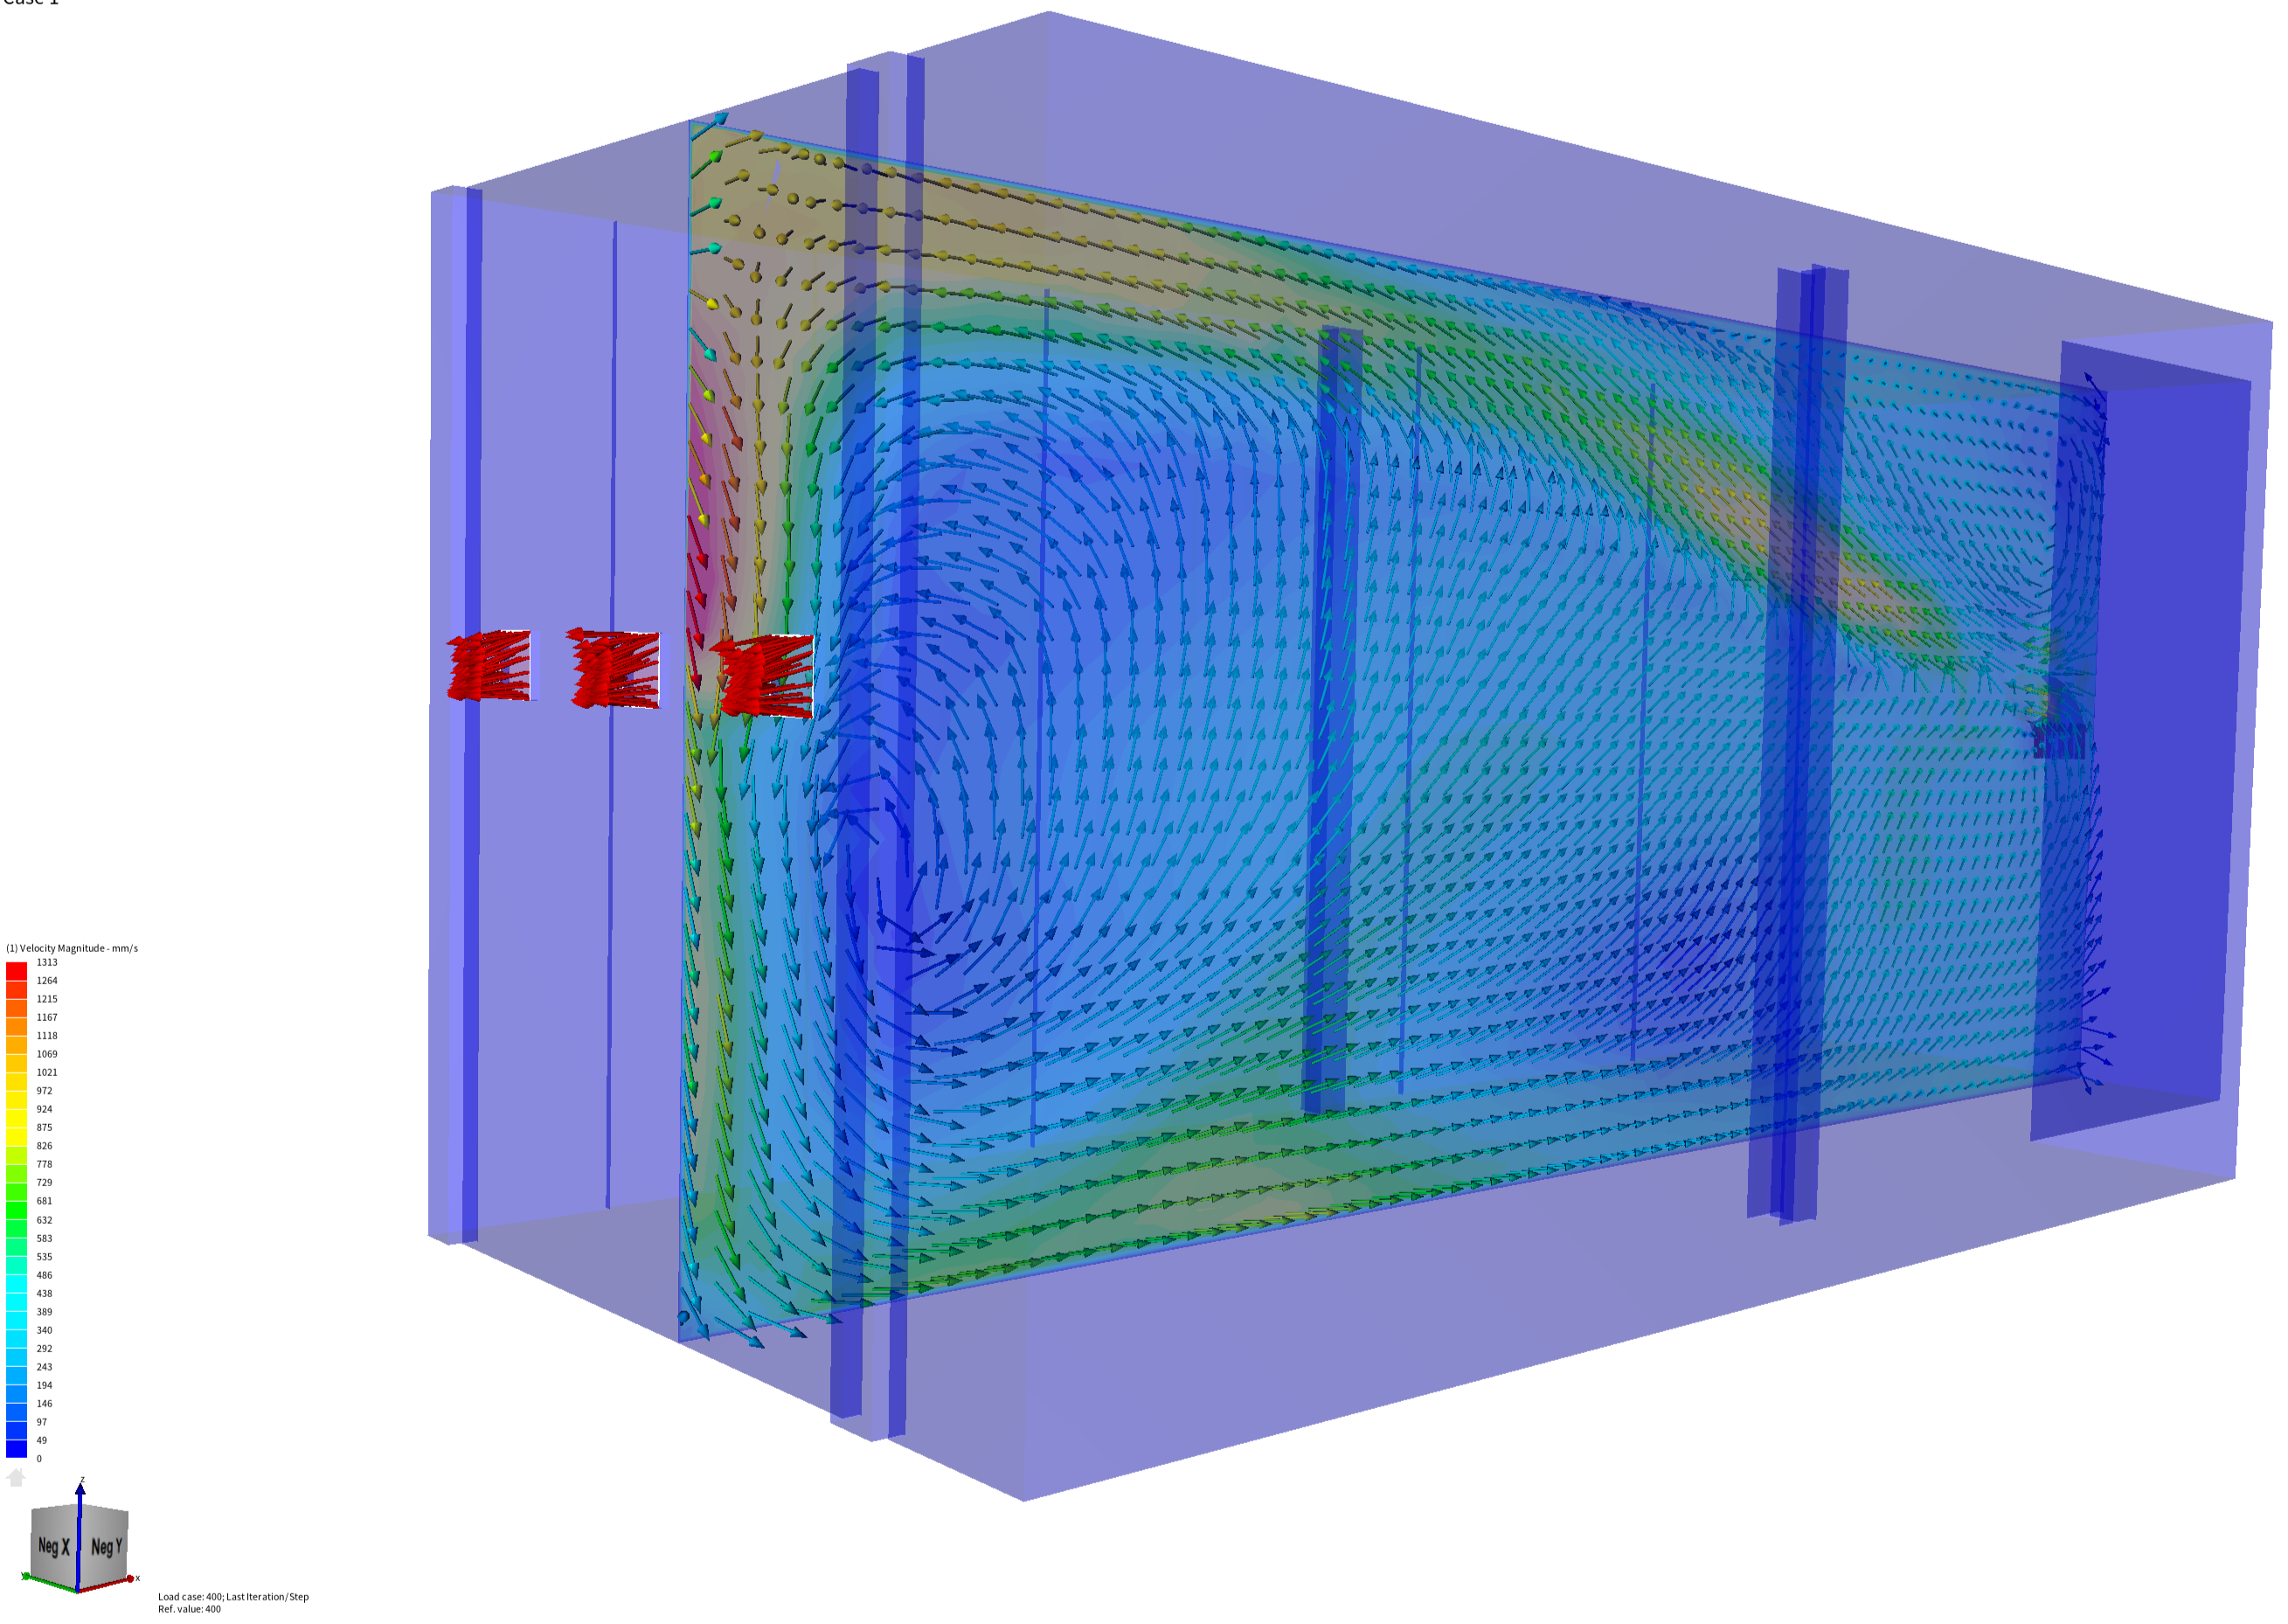
\includegraphics[width=0.92\textwidth]{figures/cfd_vectores_corte.png}
	\caption{Campo vectorial de velocidad en un corte longitudinal. Se aprecia la inyección lateral, la difusión del chorro y el patrón de recirculación en la mitad opuesta del recinto.}
	\label{fig:cfd_vectores_corte}
\end{figure}
